\documentclass[a4paper,11pt]{article}
\usepackage[T1]{fontenc}
\usepackage[utf8]{inputenc}
\usepackage{lmodern} 
\usepackage[portuguese]{babel}
\usepackage{amsmath}
\usepackage{array}
\usepackage{graphicx}			%para imagens
\usepackage{epstopdf} 			%resolve problemas eps-pdf

\usepackage{fancyhdr}			% para o cabeçalho bonito
\usepackage{caption}				%para legendas
\usepackage{subcaption}			% e sublegendas
\usepackage{placeins} 			%controlar o lugar dos floats
\pagestyle{fancy} 				% número de pag e cabeçalho
\usepackage{txfonts} 			%fontes bonitas? acho que para o título
\usepackage[usenames]{color} 	% algo com gunplot e eps
\graphicspath{{./images/}{./graph/}}		% procura imagens nessa pasta
%\usepackage{epsf} 			%%para colocar .ps 


\newcommand{\HRule}{\rule{\linewidth}{0.5mm}}


%@@@@@@@@@@@@@@@@      Cabeçalho de cada página      @@@@@@@@@@@@@@@@@@@@@@

\setlength{\headheight}{25pt}%compila sem erro
	\fancyhead{}
	\fancyfoot{}
	\fancyhead[R]{Física Experimental 4}%direito superior
	\fancyhead[L]{
\includegraphics[height=0.25in]{./images/logo_unb.pdf}}%esquerda superior
	\fancyfoot[C]{\thepage}%baixo centro
%E: Even page, O: Odd page, L: Left field, C: Center field, R: Right field, H: Header, F: Footer
% em documentos com dois lados use LO, RO. como esse documento não tem lados essa opção é inútil
\newcommand\undermat[2]{%
  \makebox[0pt][l]{$\smash{\underbrace{\phantom{%
    \begin{matrix}#2\end{matrix}}}_{\text{$#1$}}}$}#2}

\begin{document}
\begin{titlepage}
\begin{center}

% Upper part of the page. The '~' is needed because \\
% only works if a paragraph has started.

\includegraphics[width=\textwidth]{logo_unb.pdf}~\\[1cm]

\Huge Física Experimental 4\\[0.5cm]

\huge Experimento III

% Title
\HRule \\[0.4cm]
{ \huge \bfseries  Decaimento da Intensidade Luminosa e Coeficientes de Absorção e Reflexão}\\[0.4cm]

\HRule \\[0.5cm]

{\large \today}


\vfill %%o que vier depois vai ao fim da páginda


% Author and supervisor

	\begin{center} \large
		\begin{tabular}{llr} \
		& & \\[0.05cm]		
		Professora & Nadia Maria de Liz Koche & \\
		
		Alunos:& & \\
		& Juarez A.S.F 					& 11/0032829\\
		& Sérgio Fernandes da Silva Reis & 11/0140257\\
		& Jedhai Pimentel				& 09/0007883\\	[0.05cm]	
		\end{tabular}

	
	\end{center}


\end{center}
\end{titlepage}

\newpage
\thispagestyle{empty}
\mbox{ }
\newpage
\tableofcontents

\newpage

%@@@@@@@@@@@@@@@@@@@@@@@@@@@@@@@@@@@@@@@@@@@@@@@@@@@@@@@@@@@
%@@@@@@@@@@@@@@@@      OBJETIVOS      @@@@@@@@@@@@@@@@@@@@@@
%@@@@@@@@@@@@@@@@@@@@@@@@@@@@@@@@@@@@@@@@@@@@@@@@@@@@@@@@@@@
\section{Objetivos}
\paragraph{} Estudar o decaimento da intensidade luminosa que atravessa um meio material e as diversas formas pelas quais isso ocorre. Analisar também como esse decaimento ocorre quando o meio é puramente o ar.
%@@@@@@@@@@@@@@@@@@@@@@@@@@@@@@@@@@@@@@@@@@@@@@@@@@@@@@@@@@@
%@@@@@@@@@@@@@@@        MATERIAIS         @@@@@@@@@@@@@@@@@@
%@@@@@@@@@@@@@@@@@@@@@@@@@@@@@@@@@@@@@@@@@@@@@@@@@@@@@@@@@@@
\section{Materiais}
\paragraph{} O experimento faz uso de:
\begin{itemize}
	\item[•]Fonte de luz com housing colimador
	\item[•]Fonte de alimentação
	\item[•]Suporte para filtro
	\item[•]6 filtros de vidro fume
	\item[•]1 filtro vermelho
	\item[•]1 diafragma
	\item[•]1 medidor de intensidade luminosa
	\item[•]Óleo mineral
	\item[•]Uma lente
\end{itemize} 

%@@@@@@@@@@@@@@@@@@@@@@@@@@@@@@@@@@@@@@@@@@@@@@@@@@@@@@@@@@@
%@@@@@@@@@@@@@@        INTRODUCAO       @@@@@@@@@@@@@@@@@@@@
%@@@@@@@@@@@@@@@@@@@@@@@@@@@@@@@@@@@@@@@@@@@@@@@@@@@@@@@@@@@
\newpage
\section{Introdução}
\paragraph{}Ondas transportam energia e pela 1ª lei da Termodinâmica essa energia deve ser conservada. Verificam-se diversas ocasiões no dia a dia no qual a intensidade luminosa diminui ao longo da propagação da luz, isso no entanto não contradiz a primeira lei. Primeiramente a intensidade luminosa recebida está relacionada com a media no tempo da energia por uma área e não com a energia total da onda. Além disso a onda interage com a matéria e quando isso ocorre elétrons excitados podem ficar com parte da energia original ou a onda ser espalhada em outras direções diferentes da original. Veremos alguns exemplos dessas percas de intensidade.

\paragraph{}Considere um filtro de vidro sendo iluminado, queremos estudar a fração da luz incidente que é transmitida. A luz ao atingir a superfície ar-filtro de entrada percebe uma mudança no índice de refração do meio e isso causa uma razão $R_{in}$ de reflexão. Sendo $I_0$ a intensidade que incide no vidro, apenas $I_1 = (1 - R_{in})I_0$ de fato entra no vidro. Dentro do filtro temos uma razão $A$ de absorção de intensidade devido a interação com a matéria. Da intensidade $I_1$ que entra no vidro apenas $I_2 = I_1(1 - A)$ chega ao final do filtro. Quando a onda atinge a superfície vidro-ar de saída novamente ocorre uma reflexão. Supomos que a razão de reflexão de saída $R_{out}$ é a mesma da de entrada $R_{in} = R_{out} = R$.A figura \ref{fig:1-intro-filtro} ilustra esse processo. No caso de termos  $n$ filtros em série com ar entre eles teremos esse processo $n$ vezes e a intensidade final medida será:
\begin{equation}
	\begin{array}{llllllll}
	I(n) = I_0 & \underbrace{(1 - R)	^n}_\textrm{reflexão de entrada em cada filtro}& &\cdot & \underbrace{(1 - A)^n}_\textrm{absorção em cada filtro} &\cdot & \underbrace{(1 - R)^n}_\textrm{reflexão de saída em cada filtro} \\
		\end{array}
	\label{eq:intro-sem-oleo}
\end{equation} 
%\underbrace{\underbrace{a + b}_\textrm{brace 1} + c + d}_\textrm{brace 2}= e
\paragraph{}Se medirmos a intensidade de luz após esses n filtros observaremos não só a perca por absorção mas também por reflexão. Suponha agora que os filtros estivessem juntos, sem ar entre eles. Nesse caso teríamos apenas reflexão na entrada do primeiro filtro e na saída do último e a intensidade medida seria:
\begin{equation}
	\begin{array}{llllllll}
	I'(n) = I_0 & \underbrace{(1 - R)}_\textrm{reflexão de entrada no 1º filtro}& &\cdot & \underbrace{(1 - A)^n}_\textrm{absorção em cada filtro} &\cdot & \underbrace{(1 - R)}_\textrm{reflexão de saída no último filtro} \\
		\end{array}
	\label{eq:intro-com-oleo}
\end{equation} 

\paragraph{}Observe que se em vez de as placas estarem grudadas tivermos um material com mesmo índice de refração que os filtros - óleo mineral por exemplo -  permeando o espaço entre estes os efeitos relativos à reflexão serão os mesmos e a fórmula \ref{eq:intro-com-oleo} é válida.  Essas duas medidas nos ajudarão a determinar R e A. Defina a fração de luz transmitida T(n) por n filtros como:
\footnote{Para o caso sem óleo definimos também o coeficiente de transmissão por filtro T como segue: $I(n) = T^n I_0$, ou $T(n) = T^n $. Ele mede a perca total - incluindo reflexões e absorção - por filtro.}
\begin{equation}
	T(n) = \frac{I(n)}{I_0} 
\end{equation}
onde I(n) é a intensidade medida após a onda passar por n filtros e $I_0$ é a intensidade inicial de luz. Calculamos a razão entre os coeficiente $T(n)$ da primeira (sem óleo) e $T'(n)$da segunda situação (com óleo) e tiramos o log. Obtemos:
\begin{equation}
	\begin{array}{lll}
	\log \left( \frac{T(n)}{T'(n)} \right)  = &  \log \left( \frac{ \frac{(1 - R)^{2n}(1 - A)^n I_0}{I_0}}{\frac{(1 - R)^2(1 - A)^n I_0}{I_0}} \right) = &  \log \left( (1 - R)^{2n - 2} \right) \\ & & = \underbrace{(2\log (1 -R))}_\textrm{coef. angular} n \underbrace{- 2\log (1 -R)}_\textrm{coef. linear} 
		\end{array}
	\label{eq:intro-obtendo-R}
\end{equation}
\paragraph{}Podemos então obter R a partir do coeficiente angular da reta do gráfico mono-log de $\frac{T(n)}{T'(n)}$ por n. Conhecendo R podemos usar a relação \ref{eq:intro-sem-oleo} ou \ref{eq:intro-com-oleo} para obter A.

\paragraph{}Os coeficientes calculados até agora medem uma razão de intensidade transmitida, absorvida ou refletida. Queremos determinar um coeficiente de absorção $\alpha$ ou extinção $\xi$ que meça o decaimento exponencial da intensidade segundo a fórmula:
\begin{equation}
	I(x) = I_0 e^{- c x}
	\label{eq:intro-intensidade-vs-x}
\end{equation}

\paragraph{}Caso usemos $I_0$ como intensidade incidente mediremos o $c = \xi$ que engloba todas as percas, caso usemos a intensidade que de fato entra no meio obteremos $c = \alpha$. Note que é difícil saber essa intensidade que entra no vidro mas podemos determinar $\alpha$ indiretamente. Considere que na fórmula \ref{eq:intro-intensidade-vs-x} estejamos usando a intensidade que entra no filtro e seja $x_L$ o comprimento de um filtro. Nesse caso:
 $e^{-\alpha x_L} = \frac{I(x_L)}{I_0}$. Agora, a razão de absorção A é:
  \begin{equation}
     A = \frac{\overbrace{I_0 - I(x_L)}^\textrm{variação da intensidade}}{\underbrace{I_0}_\textrm{intensidade que entra no filtro}} = 1 - e^{-\alpha x_L}
	\label{eq:intro-achando-alpha}	
	\end{equation}
\paragraph{}Dessa forma, conhecendo o comprimento $x_L$ de um filtro e tendo achado a razão de absorção A podemos determinar $\alpha$ o coeficiente de absorção do filtro utilizado.

\paragraph{}A intensidade de luz também diminui na propagação pelo vácuo sem que haja meio material para absorver, dispersar ou refletir. Nesse caso a diminuição se dá pelo aumento da área coberta pela frente de onda. Se a luz é pontual então a frente de onda é esférica e a área coberta aumenta com o quadrado do raio. Assim, a mesma energia tem que se distribuir por uma maior área e a intensidade luminosa percebida(energia por área por tempo) diminui com a distancia. Veja a figura \ref{fig:2-intro-vacuo} para ilustração, a concentração de raios passando por uma mesma área diminui a medida que nos afastamos da fonte pontual. 
\FloatBarrier
\begin{figure}[!htp]
	\begin{subfigure}[!htp]{0.3\textwidth}
		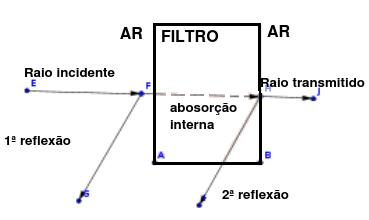
\includegraphics[scale= 0.6]{./fig:1-intro.jpeg}
		\caption{em meio material}
		\label{fig:1-intro-filtro}
	\end{subfigure}
	\hspace{2 cm}
	\begin{subfigure}[!htp]{0.3\textwidth}
		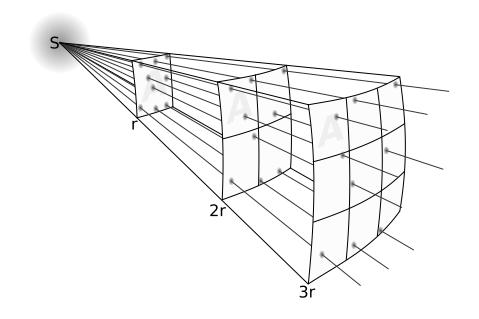
\includegraphics[scale= 0.4]{./fig:2-intro.jpeg}
		\caption{pela distância}
		\label{fig:2-intro-vacuo}
	\end{subfigure}
	\caption{Diminuição da Intensidade Luminosa}
\end{figure}
\FloatBarrier
%@@@@@@@@@@@@@@@@@@@@@@@@@@@@@@@@@@@@@@@@@@@@@@@@@@@@@@@@@@@
%@@@@@@@@@@@@       PROCEDIMENTOS        @@@@@@@@@@@@@@@@@@@
%@@@@@@@@@@@@@@@@@@@@@@@@@@@@@@@@@@@@@@@@@@@@@@@@@@@@@@@@@@@
\section{Procedimentos}
\subsection{Determinação dos coeficientes}
\paragraph{}Monta-se o banco ótico como na figura \ref{fig:proced-1} sem filtros. A lente e o diafragma são posicionados de forma a focalizar toda a área do detetor. A fonte é ligada e mede-se a intensidade $I_0$ medida no detetor. Um a um os filtros são colocados no suporte e para cada filtro adicionado anota-se a medida de intensidade de luz. Esse procedimento é refeito mas agora entre um filtro e outro pinga-se uma gota de óleo mineral que é espalhada homogeneamente pela superfície de contato.

\subsection{Medindo o decaimento da intensidade com a distância no ar}
\paragraph{}Monta-se o banco ótico como na figura \ref{fig:proced-2}. Retira-se a lente colimadora do housing e faz-se variar a distância do detetor à fonte anotando-se a intensidade medida e a distância em cada etapa. Deve-se tomar cuidado para medir a distância a partir da lâmpada da fonte e não do housing. As medidas são feitas 15 a 65 cm com saltos de 2 cm. Recoloca-se a lente colimadora no housing e as medidas são refeitas.
\FloatBarrier
\begin{figure}[!htp]
\hspace{-1 cm}
	\begin{subfigure}[!htp]{0.5\textwidth}
		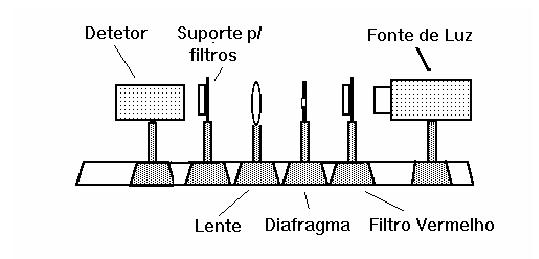
\includegraphics[scale= 0.6]{./fig:proced-montagem1.jpeg}
		\caption{procedimento 1}
		\label{fig:proced-1}
	\end{subfigure}
\hspace{2 cm}
	\begin{subfigure}[!htp]{0.5\textwidth}
		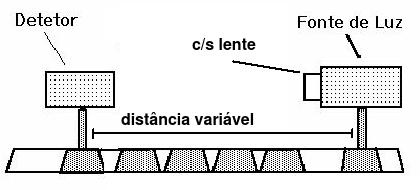
\includegraphics[scale= 0.6]{./fig:proced-montagem2.jpeg}
		\caption{procedimento 2}
		\label{fig:proced-2}
	\end{subfigure}

\caption{Procedimentos}
\end{figure}
\FloatBarrier
%@@@@@@@@@@@@@@@@@@@@@@@@@@@@@@@@@@@@@@@@@@@@@@@@@@@@@@@@@@@
%@@@@@@@@@@@@@@@@@@@       DADOS      @@@@@@@@@@@@@@@@@@@@@@
%@@@@@@@@@@@@@@@@@@@@@@@@@@@@@@@@@@@@@@@@@@@@@@@@@@@@@@@@@@@

\section{Dados}
\paragraph{}Os dados dos procedimentos 1 são mostrados nas tabelas \ref{tab:proced1-1} e \ref{tab:proced1-2}. Elas mostram ainda a razão $T(m) = \frac{I(m)}{I_0}$. Na tabela \ref{tab:proced1-3} vemos a razão $\frac{T(m)}{T'(m)}$ em função de m. Na tabela \ref{tal:proced2-1} temos os dados relativos ao procedimento 2, sendo $I_1$ a intensidade da luz medida na etapa sem lente e $I_2$ da etapa com lente.

\begin{table}[!htp]
\centering
	\begin{minipage}{0.3\textwidth}
			\begin{tabular}{|c|c|c|} \hline
				M & I(m) $\pm 5 \% $ & T(m) \\ \hline
						 0 & 281 & 1.000 \\ \hline 
		 1 & 179 & 0.637 \\ \hline 
		 2 & 112 & 0.399 \\ \hline 
		 3 & 71 & 0.253 \\ \hline 
		 4 & 46 & 0.164 \\ \hline 
		 5 & 29 & 0.103 \\ \hline 
		 6 & 19 & 0.068 \\ \hline 

			\end{tabular}
			\caption{sem óleo}	
			\label{tab:proced1-1}
	\end{minipage}
	\hspace{1.0 cm}
	\begin{minipage}{0.3\textwidth}
			\begin{tabular}{|c|c|c|}\hline
			M & I'(m)$ \pm 5\% $ & T'(m) \\ \hline
					 0 & 280 & 1.000 \\ \hline 
		 1 & 174 & 0.621 \\ \hline 
		 2 & 120 & 0.429 \\ \hline 
		 3 & 84 & 0.300 \\ \hline 
		 4 & 59 & 0.211 \\ \hline 
		 5 & 40 & 0.143 \\ \hline 
		 6 & 29 & 0.104 \\ \hline

			\end{tabular}
			\caption{com óleo}
			\label{tab:proced1-2}
	\end{minipage}

\hspace{-4.5 cm}
	\begin{minipage}{0.3\textwidth}
			\begin{tabular}{|c|c|}\hline
			M & $\frac{T(m)}{T'(m)}$  \\ \hline
					 1 & 1.026 \\ \hline 
		 2 & 0.930 \\ \hline 
		 3 & 0.843 \\ \hline 
		 4 & 0.777 \\ \hline 
		 5 & 0.720 \\ \hline 
		 6& 0.654 \\ \hline 
		 6 & 0.654 \\ \hline 

			\end{tabular}
			\caption{$\frac{T(m)}{T'(m)} \times m$}
			\label{tab:proced1-3}
	\end{minipage}	
	\caption*{}
\end{table}

\begin{table}
	\centering
	\begin{tabular}{|c|c|c|} \hline
		x(cm) $\pm 0.05$cm & $I_1(x) \pm 5\%$ & $I_2(x) \pm 5\%$ \\ \hline		
				 15.00 & 7000 & 22000 \\ \hline 
		 17.00 & 5300 & 19500 \\ \hline 
		 19.00 & 4130 & 17200 \\ \hline 
		 21.00 & 3180 & 15000 \\ \hline 
		 23.00 & 2520 & 13400 \\ \hline 
		 25.00 & 2100 & 11950 \\ \hline 
		 27.00 & 1740 & 10790 \\ \hline 
		 29.00 & 1520 & 9900\\ \hline 
		 31.00 & 1289 & 9050\\ \hline 
		 33.00 & 1116 & 8300\\ \hline 
		 35.00 & 985& 7700 \\ \hline 
		 37.00 & 862& 6990 \\ \hline 
		 39.00 & 783& 6500 \\ \hline 
		 41.00 & 705& 6000 \\ \hline 
		 43.00 & 638& 5580 \\ \hline 
		 45.00 & 576& 5280 \\ \hline 
		 47.00 & 516& 4950 \\ \hline 
		 49.00 & 475& 4670 \\ \hline 
		 51.00 & 460& 4380 \\ \hline 
		 53.00 & 419& 4160 \\ \hline 
		 55.00 & 387& 3970 \\ \hline 
		 57.00 & 360& 3720 \\ \hline 
		 59.00 & 334& 3590 \\ \hline 
		 61.00 & 325& 3420 \\ \hline 
		 63.00 & 320& 3260 \\ \hline 
		 65.00 & 303& 3180 \\ \hline 

	\end{tabular}
	\caption{Intensidade como função da distância}
	\label{tal:proced2-1}
\end{table}

%@@@@@@@@@@@@@@@@@@@@@@@@@@@@@@@@@@@@@@@@@@@@@@@@@@@@@@@@@@@
%@@@@@@@@@@@@@@       Análise         @@@@@@@@@@@@@@@@@@@@@@
%@@@@@@@@@@@@@@@@@@@@@@@@@@@@@@@@@@@@@@@@@@@@@@@@@@@@@@@@@@@
\newpage
\section{Análise de Dados}
\paragraph{}Nos gráficos \ref{graph:1-1-fitted} vemos T(m) plotado em função de m. Em \ref{graph:1-1-fitted2} vemos I(x) vs x, onde I(x) é a intensidade da etapa sem óleo. No gráfico \ref{graph:1-3-fitted} temos os dados da tabela \ref{tab:proced1-3} em escala mono-log. Em \ref{graph:2-1-fitted} vemos a curva de decaimento da intensidade em função da distância no ar para o procedimento 2 etapas com lente e sem lente. Em todos os gráficos vemos também a curva obtida da regressão dos dados. Podemos agora obter algumas constantes do processo.

\paragraph{} No gráfico \ref{graph:1-1-fitted} as equação da curva regredida à forma $T(m) = \textbf{T}^m$ é:
\begin{equation}
	\begin{array}{cl}
		  T(m) = 0.634^m
 &\\	
	\end{array}
	\label{eq:1-1}
\end{equation}
comparando os termos obtemos:
\begin{displaymath}
	\begin{array}{cl}
	 \textbf{T} = 0.634 = 63.4 \% & \mbox{(Taxa de transmissão sem óleo)}
	\end{array}
\end{displaymath}


\paragraph{} No gráfico \ref{graph:1-1-fitted2} plotamos os dados da intensidade em função do comprimento que a onda percorre dentro do filtro. Para isso apenas multiplicamos o número de filtros m pelo comprimento de cada filtro $x_l = 3 mm$. A equação da curva obtida pela regressão ao decaimento exponencial $I(x) = Ae^{-cx}$ é:
\begin{displaymath}
	\begin{array}{c}
		 I(x) =281.293 e^{-0.152 x}
 \\			
	\end{array}
	\label{eq:1-2}
\end{displaymath}
\paragraph{}Nesse caso, sem óleo, estamos considerando a perda de energia por absorção e reflexão e por isso obtemos $\xi$ o coeficiente de absorção.
\begin{equation}
	\begin{array}{ll}
	\xi = 15.2 \mbox{ mm}^{-1} & \mbox{(coeficiente de extinsão sem óleo)}	
	\end{array}
\end{equation}


\paragraph{} No gráfico \ref{graph:1-3-fitted} vemos $log(\frac{T(m)}{T'(M)})$ por m. A equação da regressão linear obtida é:
\begin{equation}
	\begin{array}{rl}
		 log (\frac{T(m)}{T'(m)}) = -0.089 \cdot m + (0.106)
 & \\
	\end{array}
	\label{eq:1-3-1}
\end{equation}
\paragraph{} Comparamos os termos da regressão com a equação \ref{eq:intro-obtendo-R} da introdução para determinar \textbf{R}.
\begin{equation}
	\begin{array}{rl}
		  \textbf{R} = 1 - 10^{-\frac{0.089}{2}} &\\
		  \Rightarrow	 \textbf{R} = 9.74\% & \mbox{(coeficiente de reflexão)}
	\end{array}
	\label{eq:1-3}
\end{equation}



\paragraph{}Podemos agora calcular a fração de absorvição A pela fórmula \ref{eq:intro-sem-oleo} fazendo $I(m) = T^m$, isolando \textbf{A}, e usando os valores de \textbf{R} e \textbf{T} obtidos. 
\begin{equation}
	\begin{array}{ll}
	  T(m) = \frac{I(m)}{I_0} = (1 - \textbf{R})^{2m}(1- \textbf{A})^m = \textbf{T}^m &\\
	  \Rightarrow \textbf{A} = 1 - \frac{\textbf{T}}{(1 - \textbf{R})^2} = 1 - \frac{0.634}{1 - 0.0974} &\\
		\textbf{A} = 22.18\% & \mbox{(fração de absorção)}
	\end{array}
	\label{eq:1-4}
\end{equation}
\paragraph{}Conhecendo \textbf{A} podemos achar o coeficiente de absorção $\alpha$ usando a fórmula \ref{eq:intro-achando-alpha}:
\begin{equation}
	\begin{array}{ll}
		\alpha = -\frac{\ln(1 - A)}{x_L} = - \frac{\ln(1 - 0.2218)}{3 \mbox{mm}} & \\
		\alpha = 0.08359 \mbox{mm}^{-1} & \mbox{(coeficiente de absorção)} 
	\end{array}
	\label{eq:1-5}
\end{equation}
\paragraph{} É válido notar que a razão de absorção \textbf{A} e o coeficiente de absorçao $\alpha$ tem significados distintos apesar de semelhantes. \textbf{A} mede uma fração da intensidade que é absorvida por filtro e pode depender da geometria deste, $\alpha$ mede o decaimento como propriedade do material. Se o filtro tivesse espessura diferente é provável que \textbf{A} fosse diferente, mas $\alpha$ seria o mesmo.

\paragraph{}Comparando com os valores dos coeficientes de absorção da água e do cobre para o mesmo comprimento de onda, temos que o coeficiente do filtro é maior que o da água e muito menor do que o do cobre, já que os valores são aproximadamente $\alpha _{H_2 O} = 0,0022 \mbox{cm}^{-1}$ e $\alpha _{cu} = 10^7 \mbox{cm}^{-1}$.

\paragraph{} Passamos agora ao estudo do decaimento da intensidade  no ar no procedimento 2. Vimos no procedimento 1 que o decaimento seguiu uma função exponencial, será que o mesmo acontece com o decaimento no ar? O gráfico \ref{graph:2-1-fitted} mostra os dados plotados junto com ajustes na forma $I(x) = Ae^{-cx}$ na linha contínua e na forma $I(x) = A(x - b)^{c}$ em tracejado. Vemos que um decaimento exponencial não se adepta aos dados mas que o decaimento polinomial sim. Essa diferença na forma do decaimento pode ser explicada pela diferença na origem do decaimento. No procedimento 1 o decaimento ocorre por interação com a matéria enquanto no procedimento 2 ela ocorre principalmente pelo aumento da área coberta pela frente de onda. As equações das curvas pontilhadas são:

\begin{equation}
	\begin{array}{ll}
		 I_1(x) = 3000000 \cdot x ^{-2.243}
 & \mbox{(decaimento sem o colimador)}\\	
		 I_2(x) = 3000001.623 \cdot (x - (-5.941)) ^{-1.610} 
 & \mbox{(decaimento com o colimador)}\\		
	\end{array}
	\label{eq:1-6}
\end{equation}


\paragraph{} A primeira equação nos mostra que o a intensidade decai aproximadamente com o quadrado da distância, o que é esperado de uma fonte pontual no vácuo. O fato de o expoente de x ser -2.243 e não -2.0 não está bem claro. Talvez isso tenha ocorrido pelo fato da fonte não ser pontual, ou ainda pode ser que ocorra interação significativa da luz com ar e isso faça a intensidade cair mais rapidamente do que no caso idealizado onde aproximamos a propagação no ar como aquela no vácuo. 

\paragraph{} Em relação a segunda equação vê-se que o colimador reduz o decaimento ao diminuir o módulo do expoente de x nas equações acima. Idealmente a intensidade da luz colimada não deveria reduzir pois o colimador ideal produziria uma onda plana que ao se propagar cobriria sempre a mesma área. Além disso nota-se que a colocação do colimador faz necessário um ajuste no eixo x dos dados, isso pode ser visto no termo (x - 5.941). Isso ocorre pois as distâncias medidas foram tomadas entre o sensor de intensidade luminosa e a lâmpada emissora. A distância entre a lâmpada e a superfície externa do colimador quando acoplado ao \textit{housing} é de 6.00 cm, aproximadamente o ajuste que foi necessário. Isso indica que para o experimento com o colimador a fonte de luz deve ser considerada como a superfície externa do colimador e não a lâmpada.



\FloatBarrier
\begin{figure}[!htp]
		\begin{minipage}{\textwidth}
					% GNUPLOT: LaTeX picture with Postscript
\begingroup
  \makeatletter
  \providecommand\color[2][]{%
    \GenericError{(gnuplot) \space\space\space\@spaces}{%
      Package color not loaded in conjunction with
      terminal option `colourtext'%
    }{See the gnuplot documentation for explanation.%
    }{Either use 'blacktext' in gnuplot or load the package
      color.sty in LaTeX.}%
    \renewcommand\color[2][]{}%
  }%
  \providecommand\includegraphics[2][]{%
    \GenericError{(gnuplot) \space\space\space\@spaces}{%
      Package graphicx or graphics not loaded%
    }{See the gnuplot documentation for explanation.%
    }{The gnuplot epslatex terminal needs graphicx.sty or graphics.sty.}%
    \renewcommand\includegraphics[2][]{}%
  }%
  \providecommand\rotatebox[2]{#2}%
  \@ifundefined{ifGPcolor}{%
    \newif\ifGPcolor
    \GPcolorfalse
  }{}%
  \@ifundefined{ifGPblacktext}{%
    \newif\ifGPblacktext
    \GPblacktexttrue
  }{}%
  % define a \g@addto@macro without @ in the name:
  \let\gplgaddtomacro\g@addto@macro
  % define empty templates for all commands taking text:
  \gdef\gplbacktext{}%
  \gdef\gplfronttext{}%
  \makeatother
  \ifGPblacktext
    % no textcolor at all
    \def\colorrgb#1{}%
    \def\colorgray#1{}%
  \else
    % gray or color?
    \ifGPcolor
      \def\colorrgb#1{\color[rgb]{#1}}%
      \def\colorgray#1{\color[gray]{#1}}%
      \expandafter\def\csname LTw\endcsname{\color{white}}%
      \expandafter\def\csname LTb\endcsname{\color{black}}%
      \expandafter\def\csname LTa\endcsname{\color{black}}%
      \expandafter\def\csname LT0\endcsname{\color[rgb]{1,0,0}}%
      \expandafter\def\csname LT1\endcsname{\color[rgb]{0,1,0}}%
      \expandafter\def\csname LT2\endcsname{\color[rgb]{0,0,1}}%
      \expandafter\def\csname LT3\endcsname{\color[rgb]{1,0,1}}%
      \expandafter\def\csname LT4\endcsname{\color[rgb]{0,1,1}}%
      \expandafter\def\csname LT5\endcsname{\color[rgb]{1,1,0}}%
      \expandafter\def\csname LT6\endcsname{\color[rgb]{0,0,0}}%
      \expandafter\def\csname LT7\endcsname{\color[rgb]{1,0.3,0}}%
      \expandafter\def\csname LT8\endcsname{\color[rgb]{0.5,0.5,0.5}}%
    \else
      % gray
      \def\colorrgb#1{\color{black}}%
      \def\colorgray#1{\color[gray]{#1}}%
      \expandafter\def\csname LTw\endcsname{\color{white}}%
      \expandafter\def\csname LTb\endcsname{\color{black}}%
      \expandafter\def\csname LTa\endcsname{\color{black}}%
      \expandafter\def\csname LT0\endcsname{\color{black}}%
      \expandafter\def\csname LT1\endcsname{\color{black}}%
      \expandafter\def\csname LT2\endcsname{\color{black}}%
      \expandafter\def\csname LT3\endcsname{\color{black}}%
      \expandafter\def\csname LT4\endcsname{\color{black}}%
      \expandafter\def\csname LT5\endcsname{\color{black}}%
      \expandafter\def\csname LT6\endcsname{\color{black}}%
      \expandafter\def\csname LT7\endcsname{\color{black}}%
      \expandafter\def\csname LT8\endcsname{\color{black}}%
    \fi
  \fi
  \setlength{\unitlength}{0.0500bp}%
  \begin{picture}(7936.00,5668.00)%
    \gplgaddtomacro\gplbacktext{%
      \csname LTb\endcsname%
      \put(946,704){\makebox(0,0)[r]{\strut{} 0}}%
      \put(946,1174){\makebox(0,0)[r]{\strut{} 0.1}}%
      \put(946,1644){\makebox(0,0)[r]{\strut{} 0.2}}%
      \put(946,2114){\makebox(0,0)[r]{\strut{} 0.3}}%
      \put(946,2584){\makebox(0,0)[r]{\strut{} 0.4}}%
      \put(946,3054){\makebox(0,0)[r]{\strut{} 0.5}}%
      \put(946,3523){\makebox(0,0)[r]{\strut{} 0.6}}%
      \put(946,3993){\makebox(0,0)[r]{\strut{} 0.7}}%
      \put(946,4463){\makebox(0,0)[r]{\strut{} 0.8}}%
      \put(946,4933){\makebox(0,0)[r]{\strut{} 0.9}}%
      \put(946,5403){\makebox(0,0)[r]{\strut{} 1}}%
      \put(1078,484){\makebox(0,0){\strut{} 0}}%
      \put(2155,484){\makebox(0,0){\strut{} 1}}%
      \put(3232,484){\makebox(0,0){\strut{} 2}}%
      \put(4309,484){\makebox(0,0){\strut{} 3}}%
      \put(5385,484){\makebox(0,0){\strut{} 4}}%
      \put(6462,484){\makebox(0,0){\strut{} 5}}%
      \put(7539,484){\makebox(0,0){\strut{} 6}}%
      \put(176,3053){\makebox(0,0){\strut{}T(m)}}%
      \put(4308,154){\makebox(0,0){\strut{}m}}%
    }%
    \gplgaddtomacro\gplfronttext{%
      \csname LTb\endcsname%
      \put(4211,5230){\makebox(0,0)[r]{\strut{}T(m)}}%
      \csname LTb\endcsname%
      \put(4211,5010){\makebox(0,0)[r]{\strut{}dados}}%
    }%
    \gplbacktext
    \put(0,0){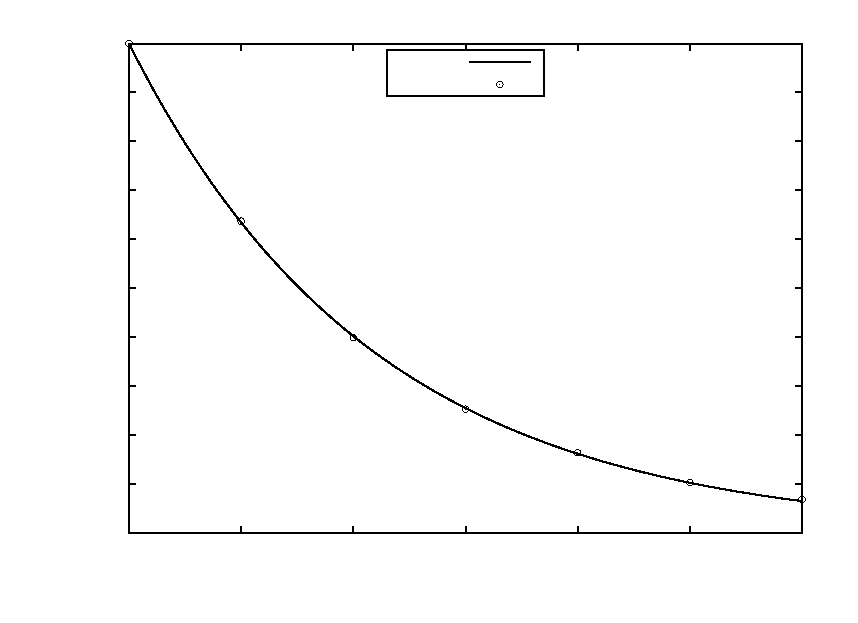
\includegraphics{1-1-fitted}}%
    \gplfronttext
  \end{picture}%
\endgroup
  
					\caption{ T(m) x m}
					\label{graph:1-1-fitted}
			
		\end{minipage}			
		\vspace{2 cm}
		\begin{minipage}{\textwidth}
				% GNUPLOT: LaTeX picture with Postscript
\begingroup
  \makeatletter
  \providecommand\color[2][]{%
    \GenericError{(gnuplot) \space\space\space\@spaces}{%
      Package color not loaded in conjunction with
      terminal option `colourtext'%
    }{See the gnuplot documentation for explanation.%
    }{Either use 'blacktext' in gnuplot or load the package
      color.sty in LaTeX.}%
    \renewcommand\color[2][]{}%
  }%
  \providecommand\includegraphics[2][]{%
    \GenericError{(gnuplot) \space\space\space\@spaces}{%
      Package graphicx or graphics not loaded%
    }{See the gnuplot documentation for explanation.%
    }{The gnuplot epslatex terminal needs graphicx.sty or graphics.sty.}%
    \renewcommand\includegraphics[2][]{}%
  }%
  \providecommand\rotatebox[2]{#2}%
  \@ifundefined{ifGPcolor}{%
    \newif\ifGPcolor
    \GPcolorfalse
  }{}%
  \@ifundefined{ifGPblacktext}{%
    \newif\ifGPblacktext
    \GPblacktexttrue
  }{}%
  % define a \g@addto@macro without @ in the name:
  \let\gplgaddtomacro\g@addto@macro
  % define empty templates for all commands taking text:
  \gdef\gplbacktext{}%
  \gdef\gplfronttext{}%
  \makeatother
  \ifGPblacktext
    % no textcolor at all
    \def\colorrgb#1{}%
    \def\colorgray#1{}%
  \else
    % gray or color?
    \ifGPcolor
      \def\colorrgb#1{\color[rgb]{#1}}%
      \def\colorgray#1{\color[gray]{#1}}%
      \expandafter\def\csname LTw\endcsname{\color{white}}%
      \expandafter\def\csname LTb\endcsname{\color{black}}%
      \expandafter\def\csname LTa\endcsname{\color{black}}%
      \expandafter\def\csname LT0\endcsname{\color[rgb]{1,0,0}}%
      \expandafter\def\csname LT1\endcsname{\color[rgb]{0,1,0}}%
      \expandafter\def\csname LT2\endcsname{\color[rgb]{0,0,1}}%
      \expandafter\def\csname LT3\endcsname{\color[rgb]{1,0,1}}%
      \expandafter\def\csname LT4\endcsname{\color[rgb]{0,1,1}}%
      \expandafter\def\csname LT5\endcsname{\color[rgb]{1,1,0}}%
      \expandafter\def\csname LT6\endcsname{\color[rgb]{0,0,0}}%
      \expandafter\def\csname LT7\endcsname{\color[rgb]{1,0.3,0}}%
      \expandafter\def\csname LT8\endcsname{\color[rgb]{0.5,0.5,0.5}}%
    \else
      % gray
      \def\colorrgb#1{\color{black}}%
      \def\colorgray#1{\color[gray]{#1}}%
      \expandafter\def\csname LTw\endcsname{\color{white}}%
      \expandafter\def\csname LTb\endcsname{\color{black}}%
      \expandafter\def\csname LTa\endcsname{\color{black}}%
      \expandafter\def\csname LT0\endcsname{\color{black}}%
      \expandafter\def\csname LT1\endcsname{\color{black}}%
      \expandafter\def\csname LT2\endcsname{\color{black}}%
      \expandafter\def\csname LT3\endcsname{\color{black}}%
      \expandafter\def\csname LT4\endcsname{\color{black}}%
      \expandafter\def\csname LT5\endcsname{\color{black}}%
      \expandafter\def\csname LT6\endcsname{\color{black}}%
      \expandafter\def\csname LT7\endcsname{\color{black}}%
      \expandafter\def\csname LT8\endcsname{\color{black}}%
    \fi
  \fi
  \setlength{\unitlength}{0.0500bp}%
  \begin{picture}(7936.00,5668.00)%
    \gplgaddtomacro\gplbacktext{%
      \csname LTb\endcsname%
      \put(946,704){\makebox(0,0)[r]{\strut{} 0}}%
      \put(946,1487){\makebox(0,0)[r]{\strut{} 50}}%
      \put(946,2270){\makebox(0,0)[r]{\strut{} 100}}%
      \put(946,3054){\makebox(0,0)[r]{\strut{} 150}}%
      \put(946,3837){\makebox(0,0)[r]{\strut{} 200}}%
      \put(946,4620){\makebox(0,0)[r]{\strut{} 250}}%
      \put(946,5403){\makebox(0,0)[r]{\strut{} 300}}%
      \put(1078,484){\makebox(0,0){\strut{} 0}}%
      \put(1796,484){\makebox(0,0){\strut{} 2}}%
      \put(2514,484){\makebox(0,0){\strut{} 4}}%
      \put(3232,484){\makebox(0,0){\strut{} 6}}%
      \put(3950,484){\makebox(0,0){\strut{} 8}}%
      \put(4667,484){\makebox(0,0){\strut{} 10}}%
      \put(5385,484){\makebox(0,0){\strut{} 12}}%
      \put(6103,484){\makebox(0,0){\strut{} 14}}%
      \put(6821,484){\makebox(0,0){\strut{} 16}}%
      \put(7539,484){\makebox(0,0){\strut{} 18}}%
      \put(176,3053){\makebox(0,0){\strut{}I(x)}}%
      \put(4308,154){\makebox(0,0){\strut{}x}}%
    }%
    \gplgaddtomacro\gplfronttext{%
      \csname LTb\endcsname%
      \put(4211,5230){\makebox(0,0)[r]{\strut{}dados}}%
    }%
    \gplbacktext
    \put(0,0){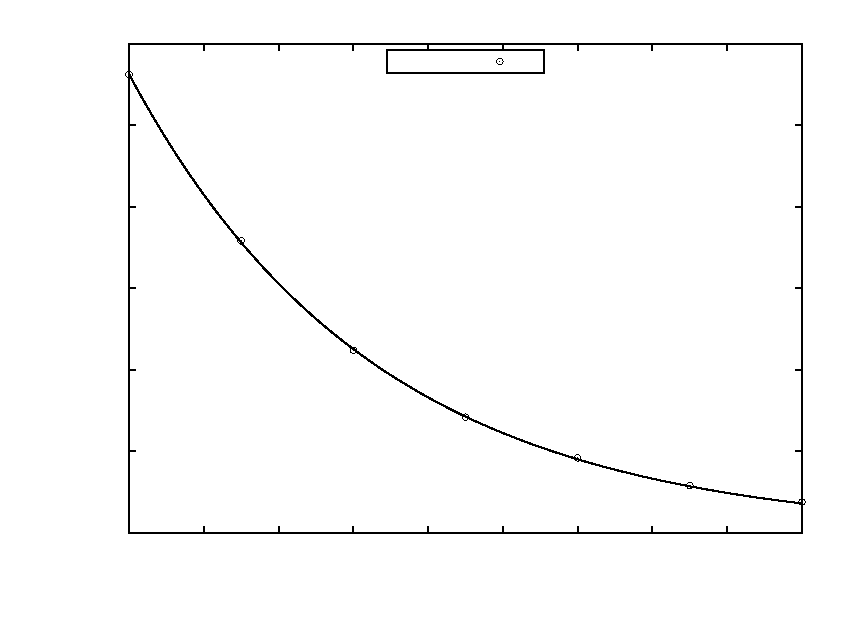
\includegraphics{1-1-fitted2}}%
    \gplfronttext
  \end{picture}%
\endgroup

				\caption{I(x) x x}
				\label{graph:1-1-fitted2}
		\end{minipage}
		\caption{Dados e regressões do procedimento 1:sem óleo}
\end{figure}
\FloatBarrier
\FloatBarrier
\vspace{-3 cm}
\begin{figure}[!htp]
		\begin{minipage}{\textwidth}	
					% GNUPLOT: LaTeX picture with Postscript
\begingroup
  \makeatletter
  \providecommand\color[2][]{%
    \GenericError{(gnuplot) \space\space\space\@spaces}{%
      Package color not loaded in conjunction with
      terminal option `colourtext'%
    }{See the gnuplot documentation for explanation.%
    }{Either use 'blacktext' in gnuplot or load the package
      color.sty in LaTeX.}%
    \renewcommand\color[2][]{}%
  }%
  \providecommand\includegraphics[2][]{%
    \GenericError{(gnuplot) \space\space\space\@spaces}{%
      Package graphicx or graphics not loaded%
    }{See the gnuplot documentation for explanation.%
    }{The gnuplot epslatex terminal needs graphicx.sty or graphics.sty.}%
    \renewcommand\includegraphics[2][]{}%
  }%
  \providecommand\rotatebox[2]{#2}%
  \@ifundefined{ifGPcolor}{%
    \newif\ifGPcolor
    \GPcolorfalse
  }{}%
  \@ifundefined{ifGPblacktext}{%
    \newif\ifGPblacktext
    \GPblacktexttrue
  }{}%
  % define a \g@addto@macro without @ in the name:
  \let\gplgaddtomacro\g@addto@macro
  % define empty templates for all commands taking text:
  \gdef\gplbacktext{}%
  \gdef\gplfronttext{}%
  \makeatother
  \ifGPblacktext
    % no textcolor at all
    \def\colorrgb#1{}%
    \def\colorgray#1{}%
  \else
    % gray or color?
    \ifGPcolor
      \def\colorrgb#1{\color[rgb]{#1}}%
      \def\colorgray#1{\color[gray]{#1}}%
      \expandafter\def\csname LTw\endcsname{\color{white}}%
      \expandafter\def\csname LTb\endcsname{\color{black}}%
      \expandafter\def\csname LTa\endcsname{\color{black}}%
      \expandafter\def\csname LT0\endcsname{\color[rgb]{1,0,0}}%
      \expandafter\def\csname LT1\endcsname{\color[rgb]{0,1,0}}%
      \expandafter\def\csname LT2\endcsname{\color[rgb]{0,0,1}}%
      \expandafter\def\csname LT3\endcsname{\color[rgb]{1,0,1}}%
      \expandafter\def\csname LT4\endcsname{\color[rgb]{0,1,1}}%
      \expandafter\def\csname LT5\endcsname{\color[rgb]{1,1,0}}%
      \expandafter\def\csname LT6\endcsname{\color[rgb]{0,0,0}}%
      \expandafter\def\csname LT7\endcsname{\color[rgb]{1,0.3,0}}%
      \expandafter\def\csname LT8\endcsname{\color[rgb]{0.5,0.5,0.5}}%
    \else
      % gray
      \def\colorrgb#1{\color{black}}%
      \def\colorgray#1{\color[gray]{#1}}%
      \expandafter\def\csname LTw\endcsname{\color{white}}%
      \expandafter\def\csname LTb\endcsname{\color{black}}%
      \expandafter\def\csname LTa\endcsname{\color{black}}%
      \expandafter\def\csname LT0\endcsname{\color{black}}%
      \expandafter\def\csname LT1\endcsname{\color{black}}%
      \expandafter\def\csname LT2\endcsname{\color{black}}%
      \expandafter\def\csname LT3\endcsname{\color{black}}%
      \expandafter\def\csname LT4\endcsname{\color{black}}%
      \expandafter\def\csname LT5\endcsname{\color{black}}%
      \expandafter\def\csname LT6\endcsname{\color{black}}%
      \expandafter\def\csname LT7\endcsname{\color{black}}%
      \expandafter\def\csname LT8\endcsname{\color{black}}%
    \fi
  \fi
  \setlength{\unitlength}{0.0500bp}%
  \begin{picture}(7936.00,5668.00)%
    \gplgaddtomacro\gplbacktext{%
      \csname LTb\endcsname%
      \put(946,704){\makebox(0,0)[r]{\strut{}-0.5}}%
      \put(946,1375){\makebox(0,0)[r]{\strut{}-0.4}}%
      \put(946,2047){\makebox(0,0)[r]{\strut{}-0.3}}%
      \put(946,2718){\makebox(0,0)[r]{\strut{}-0.2}}%
      \put(946,3389){\makebox(0,0)[r]{\strut{}-0.1}}%
      \put(946,4060){\makebox(0,0)[r]{\strut{} 0}}%
      \put(946,4732){\makebox(0,0)[r]{\strut{} 0.1}}%
      \put(946,5403){\makebox(0,0)[r]{\strut{} 0.2}}%
      \put(1078,484){\makebox(0,0){\strut{} 0}}%
      \put(2155,484){\makebox(0,0){\strut{} 1}}%
      \put(3232,484){\makebox(0,0){\strut{} 2}}%
      \put(4309,484){\makebox(0,0){\strut{} 3}}%
      \put(5385,484){\makebox(0,0){\strut{} 4}}%
      \put(6462,484){\makebox(0,0){\strut{} 5}}%
      \put(7539,484){\makebox(0,0){\strut{} 6}}%
      \put(176,3053){\makebox(0,0){\strut{}$log(\frac{T(m)}{T'(m)}$)}}%
      \put(4308,154){\makebox(0,0){\strut{}m}}%
    }%
    \gplgaddtomacro\gplfronttext{%
      \csname LTb\endcsname%
      \put(4211,5230){\makebox(0,0)[r]{\strut{}dados}}%
    }%
    \gplbacktext
    \put(0,0){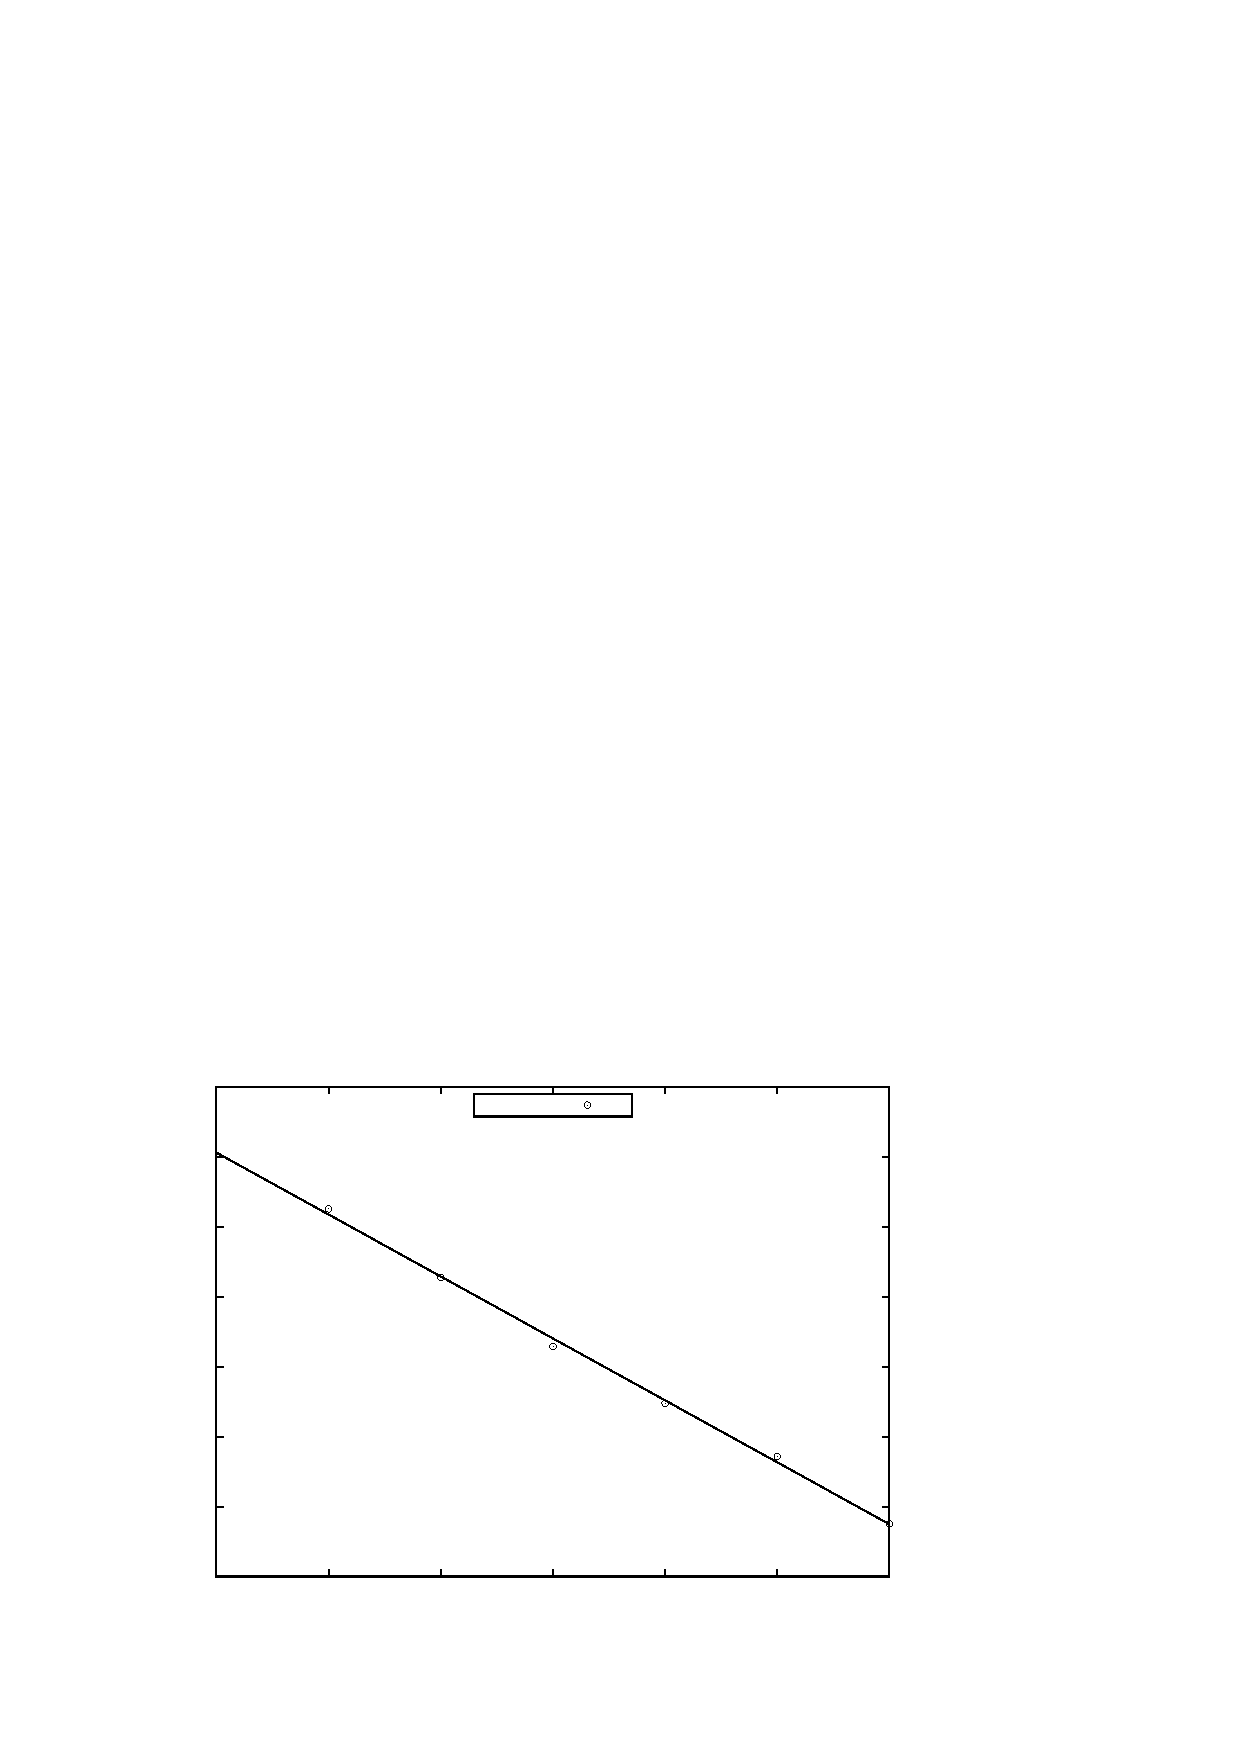
\includegraphics{1-3-fitted}}%
    \gplfronttext
  \end{picture}%
\endgroup
  
					\caption{Regressão dos dado da tabela \ref{tab:proced1-3}}
					\label{graph:1-3-fitted}
		\end{minipage}	

		\begin{minipage}{\textwidth}
				% GNUPLOT: LaTeX picture with Postscript
\begingroup
  \makeatletter
  \providecommand\color[2][]{%
    \GenericError{(gnuplot) \space\space\space\@spaces}{%
      Package color not loaded in conjunction with
      terminal option `colourtext'%
    }{See the gnuplot documentation for explanation.%
    }{Either use 'blacktext' in gnuplot or load the package
      color.sty in LaTeX.}%
    \renewcommand\color[2][]{}%
  }%
  \providecommand\includegraphics[2][]{%
    \GenericError{(gnuplot) \space\space\space\@spaces}{%
      Package graphicx or graphics not loaded%
    }{See the gnuplot documentation for explanation.%
    }{The gnuplot epslatex terminal needs graphicx.sty or graphics.sty.}%
    \renewcommand\includegraphics[2][]{}%
  }%
  \providecommand\rotatebox[2]{#2}%
  \@ifundefined{ifGPcolor}{%
    \newif\ifGPcolor
    \GPcolorfalse
  }{}%
  \@ifundefined{ifGPblacktext}{%
    \newif\ifGPblacktext
    \GPblacktexttrue
  }{}%
  % define a \g@addto@macro without @ in the name:
  \let\gplgaddtomacro\g@addto@macro
  % define empty templates for all commands taking text:
  \gdef\gplbacktext{}%
  \gdef\gplfronttext{}%
  \makeatother
  \ifGPblacktext
    % no textcolor at all
    \def\colorrgb#1{}%
    \def\colorgray#1{}%
  \else
    % gray or color?
    \ifGPcolor
      \def\colorrgb#1{\color[rgb]{#1}}%
      \def\colorgray#1{\color[gray]{#1}}%
      \expandafter\def\csname LTw\endcsname{\color{white}}%
      \expandafter\def\csname LTb\endcsname{\color{black}}%
      \expandafter\def\csname LTa\endcsname{\color{black}}%
      \expandafter\def\csname LT0\endcsname{\color[rgb]{1,0,0}}%
      \expandafter\def\csname LT1\endcsname{\color[rgb]{0,1,0}}%
      \expandafter\def\csname LT2\endcsname{\color[rgb]{0,0,1}}%
      \expandafter\def\csname LT3\endcsname{\color[rgb]{1,0,1}}%
      \expandafter\def\csname LT4\endcsname{\color[rgb]{0,1,1}}%
      \expandafter\def\csname LT5\endcsname{\color[rgb]{1,1,0}}%
      \expandafter\def\csname LT6\endcsname{\color[rgb]{0,0,0}}%
      \expandafter\def\csname LT7\endcsname{\color[rgb]{1,0.3,0}}%
      \expandafter\def\csname LT8\endcsname{\color[rgb]{0.5,0.5,0.5}}%
    \else
      % gray
      \def\colorrgb#1{\color{black}}%
      \def\colorgray#1{\color[gray]{#1}}%
      \expandafter\def\csname LTw\endcsname{\color{white}}%
      \expandafter\def\csname LTb\endcsname{\color{black}}%
      \expandafter\def\csname LTa\endcsname{\color{black}}%
      \expandafter\def\csname LT0\endcsname{\color{black}}%
      \expandafter\def\csname LT1\endcsname{\color{black}}%
      \expandafter\def\csname LT2\endcsname{\color{black}}%
      \expandafter\def\csname LT3\endcsname{\color{black}}%
      \expandafter\def\csname LT4\endcsname{\color{black}}%
      \expandafter\def\csname LT5\endcsname{\color{black}}%
      \expandafter\def\csname LT6\endcsname{\color{black}}%
      \expandafter\def\csname LT7\endcsname{\color{black}}%
      \expandafter\def\csname LT8\endcsname{\color{black}}%
    \fi
  \fi
  \setlength{\unitlength}{0.0500bp}%
  \begin{picture}(7936.00,5668.00)%
    \gplgaddtomacro\gplbacktext{%
      \csname LTb\endcsname%
      \put(1210,704){\makebox(0,0)[r]{\strut{} 0}}%
      \put(1210,1375){\makebox(0,0)[r]{\strut{} 5000}}%
      \put(1210,2047){\makebox(0,0)[r]{\strut{} 10000}}%
      \put(1210,2718){\makebox(0,0)[r]{\strut{} 15000}}%
      \put(1210,3389){\makebox(0,0)[r]{\strut{} 20000}}%
      \put(1210,4060){\makebox(0,0)[r]{\strut{} 25000}}%
      \put(1210,4732){\makebox(0,0)[r]{\strut{} 30000}}%
      \put(1210,5403){\makebox(0,0)[r]{\strut{} 35000}}%
      \put(1342,484){\makebox(0,0){\strut{} 10}}%
      \put(2375,484){\makebox(0,0){\strut{} 20}}%
      \put(3408,484){\makebox(0,0){\strut{} 30}}%
      \put(4441,484){\makebox(0,0){\strut{} 40}}%
      \put(5473,484){\makebox(0,0){\strut{} 50}}%
      \put(6506,484){\makebox(0,0){\strut{} 60}}%
      \put(7539,484){\makebox(0,0){\strut{} 70}}%
      \put(176,3053){\makebox(0,0){\strut{}$I(x)$)}}%
      \put(4440,154){\makebox(0,0){\strut{}x(cm)}}%
    }%
    \gplgaddtomacro\gplfronttext{%
      \csname LTb\endcsname%
      \put(5927,5230){\makebox(0,0)[r]{\strut{}decaimento quadrático para 1}}%
      \csname LTb\endcsname%
      \put(5927,5010){\makebox(0,0)[r]{\strut{}decaimento quadrático para 2}}%
      \csname LTb\endcsname%
      \put(5927,4790){\makebox(0,0)[r]{\strut{}dados $I_1(x)$: sem colimador}}%
      \csname LTb\endcsname%
      \put(5927,4570){\makebox(0,0)[r]{\strut{}dados $I_2(x)$: com colimador}}%
      \csname LTb\endcsname%
      \put(5927,4350){\makebox(0,0)[r]{\strut{}decaimento exponencial para 1}}%
      \csname LTb\endcsname%
      \put(5927,4130){\makebox(0,0)[r]{\strut{}decaimento exponencial para 2}}%
    }%
    \gplbacktext
    \put(0,0){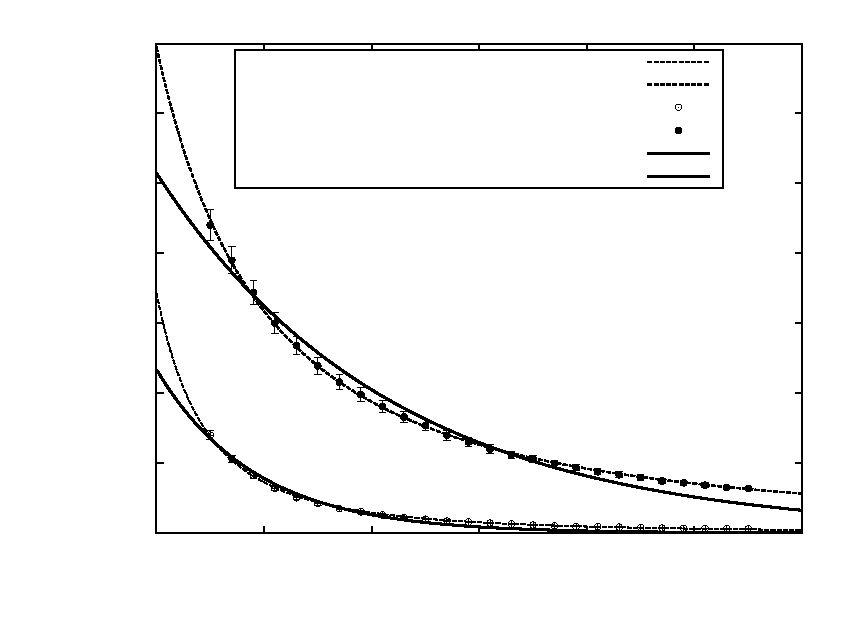
\includegraphics{2-1-fitted}}%
    \gplfronttext
  \end{picture}%
\endgroup

				\caption{Regressão dos dados do procedimento 2}
				\label{graph:2-1-fitted}
		\end{minipage}	
\end{figure}
\FloatBarrier


\newpage
%\end{comment}
%@@@@@@@@@@@@@@@@@@@@@@@@@@@@@@@@@@@@@@@@@@@@@@@@@@@@@@@@@@@
%@@@@@@@@@@@@@@       CONCLUSAO       @@@@@@@@@@@@@@@@@@@@@@
%@@@@@@@@@@@@@@@@@@@@@@@@@@@@@@@@@@@@@@@@@@@@@@@@@@@@@@@@@@@
\section{Conclusão}
\paragraph{}O experimento permitiu medir e estudar a diferença entre as várias constantes relacionadas a diminuição de intensidade luminosa devido a interação com a matéria. Para o filtro em estudo foi possível medir uma razão de 9.74\% de reflexão  e 22.18\% de absorção de intensidade. Determinou-se ainda o coeficiente de absorção do material do filtro em 0.08359 mm$^{-2}$. O estudo da intensidade luminosa com a distância percorrida no ar obteve um decaimento ligeiramente mais rápido do que o quadrático esperado, sugerindo que a interação com o ar é significativa. Por último, observamos que o uso do colimador diminui a taxa na queda da intensidade mas de forma distante da idealizada de ondas planas.

%@@@@@@@@@@@@@@@@@@@@@@@@@@@@@@@@@@@@@@@@@@@@@@@@@@@@@@@@@@@
%@@@@@@@@@@@@@@       REFERÊNCIAS     @@@@@@@@@@@@@@@@@@@@@@
%@@@@@@@@@@@@@@@@@@@@@@@@@@@@@@@@@@@@@@@@@@@@@@@@@@@@@@@@@@@
\begin{thebibliography}{9}    
	 \bibitem{fis4-serway}
  		JEWETT, J.W.; SERWAY, R.A.
  		\emph{Física para cientistas e engenheiros} volume 4 : Luz, Óptica e Física Moderna.
 		 8ª ed.
 		 São Paulo : Cengage Learning, 2012.
 		 
 	 \bibitem{fis4-halliday}
  		HALLIDAY, D.; RESNICK, R. ; WALKER.
  		\emph{Fundamentos de Física} volume 4
 		 8ª ed.
 		 Rio de Janeiro : LTC, 2009.
 	
 	\bibitem{wiki:inverso_do_quadrado}
 			Wikipedia. Inverse-square law . Disponível em: http://en.wikipedia.org/wiki/Inverse-square$\_$law. Acesso em: 29 de maio de 2013

\end{thebibliography}



\end{document}
